\subsection{Classifying}
After the websites are stored in Neo4J we want to classify each website according to subject: for example economy, politics and migration. Classifying is done in two steps: choosing the classes and actual classifying. \\
Classes can be chosen manually, however, you can also apply certain techniques to automatize results. The advantage of this that you will get unbiased results, the disadvantage is that it takes more time to make these results and it may also cause classes to be chosen which the user can't use, for example when using Google Trends  \cite{googleTrends}  results as "AFC Ajax", "Aeroflot" and "Eric Dane" may be found. The same problem occurs when searching for sub-classes. \\
For the classifying itself there are also several approaches. A standard approach is to use only the text from the websites and removing all other data. The big advantage is that it costs much less storage. Information in images may be lost however. Since we have to go over millions of pages, storage is a big issue for us therefor we choose this approach. \\
Text based classification itself can be split in classification on structured and unstructured text. Text is structured when sentences are used, meaning grammar is used. In the case of structured texts a word may say something about the next word in the sentence, therefor other techniques can be used (for example n-grams) then in case of unstructured texts.Because the text from websites can be structured as well as unstructured, we will most likely use unstructured approaches. One way to do this is by using machine learning.

\subsubsection{Defining classes}
One problem we need to solve is the problem of choosing classes. This can be done in several ways. The easiest way is to define these ourselves, however we may get better results if we used some algorithm. When using algorithms we may also decide if we want to consistently use the same classes for each pair of cities, or define the classes per pair depending on the importance. For example if Rotterdam and Vlissingen have a huge trade of fish, "fish" we be an important class of the relation between Rotterdam and Vlissingen. However if Leiden does nothing with fish, the class will be absent for the relation Rotterdam-Leiden or Vlissingen-Leiden. One way to do this is to look at the websites for each relation and apply the 'bag of words' model to check which words occur most frequently (after stemming and the removal of stop words). To make sure we don't get similar results (for example the relations 'fish' and 'fishmarket') we could remove all websites containing 'fish' and then applying the same model again.

\subsubsection{Machine Learning for classification of unstructured text}
Text based machine learning for unstructured texts is done using the 'bag of words'. This model counts how often each word is used. There are 3 libraries available which contain most steps needed. There is scikit-learn \cite{scikit-learn} and TensorFlow \cite{tensorFlow} for Python and Weka \cite{weka} for Java. Since we write our program in python, and TensorFlow is only about neural networks, we choose to use scikit-learn.
The machine learning works in 4 steps:
\begin{enumerate}
    \item \textbf{Creating a feature extractor} \\
    Given text from a website, the "features" from this text are returned. Features are the words that occur in the text and the number of occurrences. Before this data is extracted stop words (the, is, at etc) are removed and the rest of the words are stemmed meaning all words will be changed to their root-forms (features - feature, controlled - control). The program Snowball \cite{snowball_dutch} and NLKT \cite{nlkt_stemming} (which uses the snowball version) have a dutch implementation for this, although it might need to be improved a bit.
    
    Afterwards, to prepare the features for the machine learning algorithm. We need to give each feature a numeric id. Count each of these tokens. And we need to normalise the tokens. For this scikit-learn provides algorithms.
    \item \textbf{Manually labelling} \\
    For each of the classes (e.g. business, tourism, art etc) we select a few websites we know fit to that class. Here occurs the problem of defining classes which will be expanded on later. From these websites all the words will be extracted and their occurrence will be counted. Possibly some normalisation functions are applied to get better values. We call these values the weight for each word for each class. From this we create a two dimensional array with in the rows each of the websites and in the columns all different words and one extra for the class. We fill the fields with the weights or a zero if the words don't occur.
    
    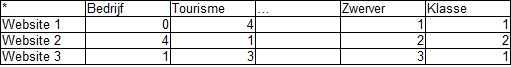
\includegraphics{classTable}
    
    \item \textbf{Generating a classifier} \\
    The array is fed to a learning algorithms. This will generate a classifier. There are a multitude of classifiers importable from Scikit-learn and TensorFlow. For choosing the classifier we make use of the Microsoft Azure Machine Learning Test Sheet \cite{MLCheatSheet}. Several factors should be taken into account when choosing an algorithm. These are:
    \begin{enumerate}
        \item Accuracy - How well the algorithm separates the websites.
        \item Training Time - How long it takes to train the algorithm.
        \item Linearity - Linear regression assumes data trends follow a straight line. This is trade-off between accuracy and speed.
        \item Number of Parameters - Adjustable parameters increase the flexibility of the algorithms. This is a trade-off between training time and accuracy.
        \item Number of Features - A large number of features can make some algorithms unfeasibly long. Especially text data (what we are using!) has a large number features. Support Vector Machines are especially well suited in this case.
        \item Special Cases - Some learning algorithms make particular assumptions about the data or the results.
    \end{enumerate}
    
    For textual data especially support vector machines are recommended, so it is most likely we will choose that machine learning algorithm. Depending on whether we have time we might do some tests before making our decision however.
    
    \item \textbf{Entering new examples} \\
    When a new (unlabelled) example (website) comes - extract the features and feed it to your classifier - it will tell you what it thinks it is (and usually - what is the probability the classifier is correct). Afterwards the classifier can be updated to include new features extracted from the example. This updating probably needs to be done a couple of times because the first few times not all features (possible words in the dutch dictionary) will be included. It is important to choose the same amount of websites for each class.
\end{enumerate}

\subsection{conclusion}
After all websites are classified and possibly sub-classified we can use that data to show the strengths of the connections between cities by counting for each class how many websites there are that contain information about both cities. 



%\subsubsection{TF-IDF}
%basic idea: 1. using training data to assign values on words - filter meaningless words - assign words with highest value as categories? 2. Do the same on training data for each category (choose a few documents manually per category) and then check for websites for which categories has the highest value.